%
% funktionen.tex -- Neue Funktionen: elliptische Integrale und Funktionen
%
% (c) 2026 Baris Catan, OST Ostschweizer Fachhochschule
%
% !TEX root = ../../buch.tex
% !TEX encoding = UTF-8
%
\section{Neue Funktionen
\label{elliptisch:section:funktionen}}
\kopfrechts{Neue Funktionen}

Der vorangegangene Abschnitt hat mit dem Vorsatz geendet, dem
Ellipsenintegral einen Namen zu geben.
Bevor wir das tun, ist zu klären, wie viele Namen wir brauchen.
Die Definition \eqref{elliptisch:equation:definition} lässt für die
rationale Funktion $R$ und das Polynom $p$ unendlich viele
Möglichkeiten zu, und für jede davon eine eigene Funktion
einzuführen wäre nutzlos.

\subsection{Der Reduktionssatz}
Die Lage ist besser, als sie aussieht.
Die elliptischen Integrale bilden zwar eine unübersehbare Menge,
aber sie unterscheiden sich nur um elementare Anteile, und was
davon übrig bleibt, sind drei feste Integrale.
\begin{satz}[Reduktionssatz]
\label{elliptisch:satz:reduktion}
Jedes elliptische Integral lässt sich als Summe elementarer
Funktionen und der drei Integrale
\begin{equation}
\int \frac{dt}{\sqrt{p(t)}},
\qquad
\int \frac{\sqrt{1-k^2t^2}}{\sqrt{1-t^2}}\,dt,
\qquad
\int \frac{dt}{(1-nt^2)\sqrt{p(t)}}
\label{elliptisch:equation:normalformen}
\end{equation}
mit dem Radikanden $p(t) = (1-t^2)(1-k^2t^2)$ und $0 < k < 1$
schreiben.
\end{satz}
Der Beweis ist bei Smirnow zu finden
\cite[Abschnitt~164, S.~506]{elliptisch:smirnow}, dieselbe Stelle
zitiert auch Müller \cite{elliptisch:mueller-spezielle}.
Er verläuft in zwei Schritten.
Zuerst wird das beliebige Polynom $p$ vom Grad $3$ oder $4$ durch
eine gebrochen lineare Substitution auf den Radikanden
$(1-t^2)(1-k^2t^2)$ gebracht, was den Modul $k$ überhaupt erst
erzeugt.
Danach wird der rationale Anteil des Integranden durch
Partialbruchzerlegung und wiederholte partielle Integration
abgebaut, bis nur noch die drei Reste in
\eqref{elliptisch:equation:normalformen} stehen.
\index{Reduktionssatz}%

Diese drei heissen elliptische Integrale erster, zweiter und
dritter Art.
Die Zahl $k$ heisst \emph{Modul}, die Zahl $n$ in der dritten Art
\emph{Charakteristik}.
\index{Modul}%
\index{Charakteristik}%
Beim Integral zweiter Art kürzt sich $\sqrt{1-k^2t^2}$ heraus, es
lässt sich also auch über dem gemeinsamen Radikanden schreiben,
\begin{equation}
\int \frac{1-k^2t^2}{\sqrt{p(t)}}\,dt
=
\int \sqrt{\frac{1-k^2t^2}{1-t^2}}\,dt.
\label{elliptisch:equation:zweiteart}
\end{equation}
Alle drei Arten haben damit denselben Radikanden, sie unterscheiden
sich nur im Zähler und im zusätzlichen Faktor $1-nt^2$.
Die dritte Art führen wir der Vollständigkeit halber mit, im
weiteren Verlauf dieses Kapitels wird sie nicht mehr gebraucht.

Eine Warnung zur Notation ist hier angebracht.
Viele Tabellenwerke und Programmbibliotheken benutzen statt des
Moduls $k$ den Parameter $m = k^2$.
In \texttt{scipy} etwa liefert erst \texttt{ellipk(k**2)} das
Integral zum Modul $k$.
Wir schreiben durchgehend $k$.

\subsection{Die vollständigen elliptischen Integrale}
Die Integrale in \eqref{elliptisch:equation:normalformen} sind
unbestimmt und legen damit keine Funktion fest.
Eine Funktion entsteht erst, wenn wir die Grenzen festnageln.
Der Radikand $p(t)$ hat bei $t = \pm 1$ eine Nullstelle, weiter als
bis $1$ lässt sich also nicht integrieren.
Genau diese Grenzen wählen wir.
\begin{definition}
\label{elliptisch:definition:vollstaendig}
Die \emph{vollständigen elliptischen Integrale} erster, zweiter und
dritter Art sind für $0 < k < 1$
\begin{equation}
\begin{aligned}
K(k)
&=
\int_0^1 \frac{dt}{\sqrt{(1-t^2)(1-k^2t^2)}},
\\
E(k)
&=
\int_0^1 \sqrt{\frac{1-k^2t^2}{1-t^2}}\,dt,
\\
\Pi(n,k)
&=
\int_0^1 \frac{dt}{(1-nt^2)\sqrt{(1-t^2)(1-k^2t^2)}}.
\end{aligned}
\label{elliptisch:equation:vollstaendig}
\end{equation}
\end{definition}
\index{elliptisches Integral!vollstandiges@vollständiges}%
\index{K@$K(k)$}%
\index{E@$E(k)$}%

Diese Gestalt heisst \emph{Jacobi-Normalform}.
Die Substitution $t = \sin\varphi$ führt auf eine zweite,
ebenso gebräuchliche Schreibweise.
Wegen $\sqrt{1-t^2} = \cos\varphi$ und $dt = \cos\varphi\,d\varphi$
ist
\begin{equation}
\frac{dt}{\sqrt{1-t^2}}
=
d\varphi,
\label{elliptisch:equation:legendresubst}
\end{equation}
und die obere Grenze $t = 1$ geht in $\varphi = \pi/2$ über.
Damit werden aus \eqref{elliptisch:equation:vollstaendig} die
Integrale
\begin{equation}
K(k)
=
\int_0^{\pi/2} \frac{d\varphi}{\sqrt{1-k^2\sin^2\varphi}},
\qquad
E(k)
=
\int_0^{\pi/2} \sqrt{1-k^2\sin^2\varphi}\,d\varphi,
\label{elliptisch:equation:legendreform}
\end{equation}
und entsprechend für $\Pi$.
Diese Gestalt heisst \emph{Legendre-Normalform}
\cite[Kapitel~11.1.2]{elliptisch:mueller-spezielle}.
\index{Jacobi-Normalform}%
\index{Legendre-Normalform}%
Beide Formen beschreiben dieselben Funktionen.
Wer in der Literatur einmal die obere Grenze $1$ und einmal
$\pi/2$ antrifft, sieht nur diesen Wechsel der Variablen.

\subsection{Randwerte und Verlauf}
$K$ und $E$ hängen stetig von $k$ ab, und an beiden Rändern des
Intervalls $0 < k < 1$ lassen sich die Werte direkt ausrechnen.
Für $k = 0$ verschwindet der Term mit $k^2$ in beiden Integralen,
und es bleibt zweimal dasselbe stehen,
\begin{equation}
K(0)
=
E(0)
=
\int_0^1 \frac{dt}{\sqrt{1-t^2}}
=
\arcsin 1
=
\frac{\pi}{2}.
\label{elliptisch:equation:randnull}
\end{equation}
Das ist der Viertelkreis, wie es sein muss.
Für $k = 1$ trennen sich die beiden.
Beim Integral zweiter Art kürzen sich Zähler und Nenner vollständig,
\begin{equation}
E(1)
=
\int_0^1 \sqrt{\frac{1-t^2}{1-t^2}}\,dt
=
\int_0^1 dt
=
1.
\label{elliptisch:equation:randeins}
\end{equation}
Beim Integral erster Art dagegen wird der Radikand zu $(1-t^2)^2$,
der Integrand also zu
\begin{equation}
\frac{1}{1-t^2}
\approx
\frac{1}{2(1-t)}
\qquad
\text{für } t \to 1,
\label{elliptisch:equation:kdivergenz}
\end{equation}
und $\int^1 dt/(1-t)$ divergiert logarithmisch.
Somit ist $K(1) = \infty$.
Wie schnell $K$ wächst, beschreibt man am besten mit dem
\emph{komplementären Modul}
\begin{equation}
k' = \sqrt{1-k^2},
\qquad
k^2 + k'^2 = 1,
\label{elliptisch:equation:kstrich}
\end{equation}
\index{Modul!komplementarer@komplementärer}%
der die elliptische Variante des Satzes von Pythagoras erfüllt und
uns von hier an begleitet.
Mit ihm gilt die Asymptotik
\begin{equation}
K(k)
\sim
\log \frac{4}{k'}
\qquad
\text{für } k \to 1
\label{elliptisch:equation:kasymptotik}
\end{equation}
\cite[Kapitel~11.1]{elliptisch:mueller-spezielle}.
Abbildung~\ref{fig:elliptisch:keplot} zeigt beide Funktionen.
\begin{figure}
\centering
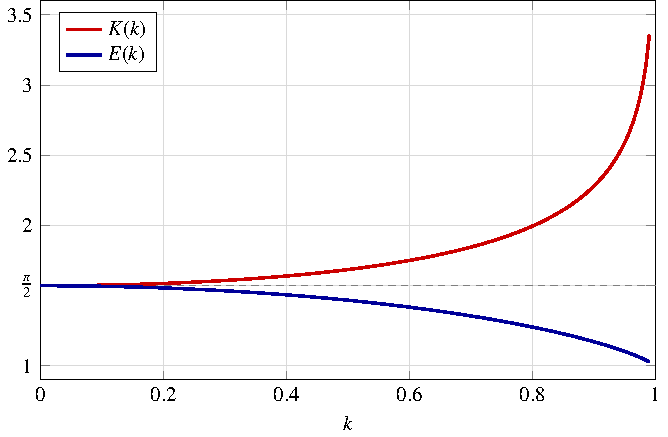
\includegraphics[width=0.72\textwidth]{papers/elliptisch/images/ke-plot.pdf}
\caption{Die vollständigen elliptischen Integrale erster und
zweiter Art.
Beide starten bei $k=0$ im gemeinsamen Wert $\pi/2$.
$E(k)$ fällt monoton auf $E(1) = 1$, während $K(k)$ monoton wächst
und für $k \to 1$ logarithmisch divergiert.
\label{fig:elliptisch:keplot}}
\end{figure}

Der Vergleich von \eqref{elliptisch:equation:legendreform} mit dem
Umfangsintegral \eqref{elliptisch:equation:umfang} zeigt, dass wir
die gesuchte Funktion bereits haben.
Das Integral zweiter Art in Legendre-Normalform ist Zeichen für
Zeichen der Ausdruck, der beim Ellipsenumfang stehen geblieben ist,
und damit gilt
\begin{equation}
U
=
4a\,E(k),
\qquad
k^2 = \frac{a^2-b^2}{a^2},
\qquad
a \ge b.
\label{elliptisch:equation:umfangE}
\end{equation}
Für den Kreis ist $k = 0$, und mit $E(0) = \pi/2$ folgt
$U = 4a\cdot\pi/2 = 2\pi a$.
Die Frage vom Anfang des Kapitels ist damit beantwortet, wenn auch
nicht durch eine elementare Formel, sondern durch eine eigens
definierte Funktion.
Dabei ist die Reihenfolge das Entscheidende.
Auch $\int dt/t$ war nicht darstellbar, solange es den Logarithmus
noch nicht gab, und erst seine Aufnahme in den Funktionsvorrat hat
das Integral lösbar gemacht.
Elementar ist also keine Eigenschaft eines Integrals an sich,
sondern eine Aussage über einen vorher festgelegten Vorrat.
